\section{Rolando}

\subsubsection{Diagrama GANTT}

El siguiente diagrama fue generado con los siguientes parametros:

\begin{enumerate}
	\item lote\_tsk: 1.tsk
	\item num\_cores: 1
	\item switch\_cost: 0
	\item sched\_class: SchedFCFS
	\item n: 10
	\item bmin: 1
	\item bmax: 10
\end{enumerate}

\begin{figure}[h]
    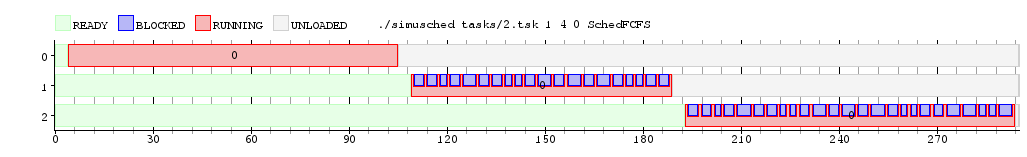
\includegraphics[width=\linewidth]{images/2_1nucleo.png}
    \label{fig:Task Consola}
    \caption{Rolando con 1 núcleo}
\end{figure}

\begin{figure}[h]
    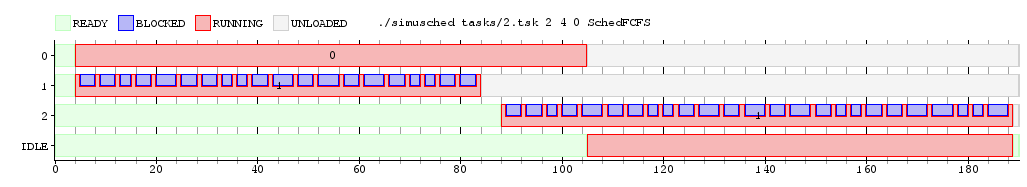
\includegraphics[width=\linewidth]{images/2_2nucleos.png}
    \label{fig:Task Consola}
    \caption{Rolando con 2 núcleos}
\end{figure}

\textbf{TODO: Explicar bien el diagrama!}